% Printed 242; principal PDF 249; Google PDF 253.
\par\clearpage
\noindent\makebox[0pt][l]{\fontsize{13}{16}\selectfont 242}\hfill{\small\textbf{REMARKS.\quad TRIGONOMETRIC POINT DETERMINATION.}}\hfill\null\par\medskip

{\small
\noindent points could be intersected. It is sufficient to observe from these points toward other points that have already been fixed, but there must be at least 3 of them. If 4 have been observed, there is a check. If these 4 do not agree, however, which is also not uncommon because a mix-up can occur quite easily, one does not know where the error lies. It is therefore better to observe toward 5 or more. . . . . In general, one cannot recommend strongly enough intersecting every point as often as is practicable, even if one does not intend to combine the intersections by the method of least squares. This guards against errors, and even a point that is neither principal nor secondary, once precisely determined, can often help establish the identity of another point. Once the coordinates have been calculated for the secondary points as well, one goes on to determine the remaining points that have been intersected. After all the\\
\makebox[0pt][r]{.\enspace}calculations are complete, \textsc{Gauss} records the results in the following log.
\[
 \overbrace{\text{\textls[120]{Krückeberg}}}^{A}
 \quad\overbrace{-71364{,}939\qquad+45842{,}386}^{B}
\]
\[
\begin{array}{@{}l@{\qquad}r@{\qquad}r@{\qquad}r@{\;}r@{\;}r@{\qquad}r@{}}
 \multicolumn{1}{c}{a}&\multicolumn{1}{c}{b}&\multicolumn{1}{c}{c}&
 \multicolumn{3}{c}{d}&\multicolumn{1}{c@{}}{e}\\
 \text{Süntel}&-70637{,}258&+37481{,}447&94^\circ&58'&27''{,}964&-0{,}885\\
 \text{Klütberg}&-63179{,}059&+41387{,}660&151&26&44{,}009&-1{,}553\\
 \text{Wittekindstein}&-80356{,}285&+71875{,}835&289&3&13{,}703&-0{,}329\\
 \text{Pagenburg}&-75427{,}470&+50454{,}707&311&22&31{,}882&+0{,}448\\
 \hline
 \multicolumn{7}{c@{}}{\text{\textls[120]{Sachsenhagen, Castle}}\;-96486{,}713\qquad+46075{,}741}\\
 \text{Wittekindstein}&-80356{,}285&+71875{,}835&237&59&11{,}516&\\
 \text{Bergkirchen}&-99061{,}252&+47440{,}144&332&4&3{,}954.&\\
 \hline
\end{array}
\]

\(A\) is the location whose coordinates are being determined. These coordinates are given under \(B\). \(a\) lists the names of the locations from which \(A\) is determined. The coordinates of those locations are given under \(b,c\), the observed azimuth under \(d\), and the difference between the azimuth calculated from the coordinates and the observed azimuth under \(e\). This last column is therefore omitted whenever we have \textls[120]{no more} data than are necessary to determine the point in question. No particular order is imposed on the points recorded in this log, but it is advisable to leave some space for adding remarks that arise later and intersections found only after calculation and entry. The points are entered in this log in the order in which they are calculated. In the tables, the intersections already used in calculation are marked so that it is easier to see which intersections are still outstanding.«

A large number of such logs are still among the posthumous papers. In the report on the work for 1844, \textsc{Gauss} says, »Each year, after processing the measurements, the results [coordinates] were entered in lists. There are sixteen such partial lists, containing a little over 3000 determinations in all. The number of points themselves may, however, be smaller by about one seventh, since many points that could be determined more precisely or reliably in a later year after new data became available appear in more than one list. . . . . For greater assurance and ease of use, I have now begun merging the partial lists into a single one, which will accordingly contain about 2600 points.« (Volume IV, p. 413).

Several typographical and computational errors have been corrected in Art. 6 of the reprint of the paper taken from the Astr. Nachr.\hfill\textsc{Krüger.}\par
\begin{center}\rule{4cm}{.4pt}\end{center}
}

% Printed 243; principal PDF 250; Google PDF 254.
\par\clearpage

\thispagestyle{empty}
\vspace*{.23\textheight}
{\centering
{\LARGE ADJUSTMENT\par}
\medskip
{\LARGE\bfseries OF SIMPLE FIGURES.\par}
}
\vfill
\noindent\hfill31\textsuperscript{*}\hspace*{.15\linewidth}\par
\vspace*{.14\textheight}

% Printed 244; principal PDF 251; Google PDF 255.
\par\clearpage

\null\thispagestyle{empty}

% Printed 245; principal PDF 252; Google PDF 256.
\par\clearpage

\thispagestyle{empty}
\vspace*{3\baselineskip}
{\centering\Large\bfseries POSTHUMOUS PAPERS AND CORRESPONDENCE.\par}
\vspace{3\baselineskip}
{\centering
[1.]\par\smallskip
Adjustment of a quadrilateral.\par}
\begin{flushleft}
\hspace*{1.8em}\(0,1,2,3\) . . . the four points\\
\hspace*{1.8em}\(01\) . . . . . . . . both the length and the direction of the line \(01\)\\
\hspace*{1.8em}\(C^{01}\), etc., adjustments that make everything consistent,
\end{flushleft}
\[
 C^{01}=\left[\tfrac12(C^{01}+C^{10})+\tfrac12(C^{01}-C^{10})=\right]S^{01}+D^{01},
\]
\noindent where
\[
 S^{01}=S^{10},\qquad D^{01}=-D^{10};
\]
{\centering etc.\par}

[Set]
\[
 \log\operatorname{hyp}
 \frac{\sin(30-31)\sin(10-12)\sin(20-23)}
      {\sin(32-30)\sin(13-10)\sin(21-20)}
 =\lambda^0
\]
\[
\begin{array}{@{}r@{\;=\;}l@{}}
 12\,.\,13\,.\sin(12-13)&T^0\\
 02\,.\,03\,.\sin(03-02)&T'\\
 03\,.\,13\,.\sin(30-31)&T''\\
 02\,.\,12\,.\sin(21-20)&T'''.
\end{array}
\]

Here \(T^0,T',T'',T'''\) denote twice the areas of the four triangles. Note that two permutations must always be made together. Thus \(T'\) is obtained from \(T^0\) by interchanging \(0\) and \(1\) and \(2\) and \(3\). We have [since \(T^0\) and \(T''\) have the opposite sign to \(T'\) and \(T'''\)]
\[
 0=T^0+T'+T''+T'''.
\]
Similarly, \(\lambda',\lambda'',\lambda'''\) are obtained from \(\lambda^0\).

% Printed 246; principal PDF 253; Google PDF 257.
\par\clearpage
\noindent\makebox[0pt][l]{\fontsize{13}{16}\selectfont 246}\hfill{\small\textbf{POSTHUMOUS PAPERS.}}\hfill\null\par\medskip

We then have
\[
\resizebox{\linewidth}{!}{\(\begin{aligned}
 {[}0={}&\lambda^0+\frac{\sin(13-12)}{\sin(10-12)\sin(13-10)}C^{10}
 -\operatorname{cotang}(10-12)\,.\,C^{12}
 -\operatorname{cotang}(13-10)\,.\,C^{13}\\
 &+\frac{\sin(21-23)}{\sin(20-23)\sin(21-20)}C^{20}
 -\operatorname{cotang}(21-20)\,.\,C^{21}
 -\operatorname{cotang}(20-23)\,.\,C^{23}\\
 &+\frac{\sin(32-31)}{\sin(30-31)\sin(32-30)}C^{30}
 -\operatorname{cotang}(30-31)\,.\,C^{31}
 -\operatorname{cotang}(32-30)\,.\,C^{32}
\end{aligned}\)}
\]
\noindent or
\[
\begin{aligned}
 0={}&\lambda^0-\frac{01^2\,.\,T^0}{T''T'''}C^{10}
 -\tfrac12\frac{01^2+12^2-02^2}{T'''}C^{12}
 -\tfrac12\frac{01^2+13^2-03^2}{T''}C^{13}\\
 &-\frac{02^2\,.\,T^0}{T'T'''}C^{20}
 -\tfrac12\frac{02^2+12^2-01^2}{T'''}C^{21}
 -\tfrac12\frac{02^2+23^2-03^2}{T'}C^{23}\\
 &-\frac{03^2\,.\,T^0}{T'T''}C^{30}
 -\tfrac12\frac{03^2+13^2-01^2}{T''}C^{31}
 -\tfrac12\frac{03^2+23^2-02^2}{T'}C^{32}
\end{aligned}
\]
\noindent or]
\[
\begin{array}{@{}r@{\;}r@{\;}l@{}}
 -T'T''T'''\lambda^0={}&-T^0T'\,.\,01^2\,.\,S^{01}&+T^0T'\,.\,01^2\,.\,D^{01}\\
 &-T^0T''\,.\,02^2\,.\,S^{02}&+T^0T''\,.\,02^2\,.\,D^{02}\\
 &-T^0T'''\,.\,03^2\,.\,S^{03}&+T^0T'''\,.\,03^2\,.\,D^{03}\\
 &-T'T'''\,.\,13^2\,.\,S^{13}&+T'T'''\,.\,(03^2-01^2)D^{13}\\
 &-T'T''\,.\,12^2\,.\,S^{21}&+T'T''\,.\,(01^2-02^2)D^{21}\\
 &-T''T'''\,.\,23^2\,.\,S^{32}&+T''T'''\,.\,(02^2-03^2)D^{32}\\
 =&\Sigma^0&+\qquad\Delta^0.
\end{array}
\]

\(\Sigma',\Sigma'',\Sigma'''\) are identically equal to \(\Sigma^0\). The quantities \(\lambda^0,\allowbreak \lambda',\allowbreak \lambda'',\allowbreak \lambda'''\) are proportional to \(T^0,\allowbreak T',\allowbreak T'',\allowbreak T'''\) once the angle sums have been adjusted. By contrast, \(\Delta',\Delta'',\Delta'''\) must become numerically equal to \(\Delta^0\) if that adjustment is preserved. In symmetric form this value is
\[
\begin{aligned}
 \tfrac14(\Delta^0+\Delta'+\Delta''+\Delta''')=\tfrac14\bigl\{&
 T^0T'D^{01}(12^2+13^2-02^2-03^2)\\
 &+T^0T''D^{02}(12^2+23^2-01^2-03^2)\\
 &+T^0T'''D^{03}(13^2+23^2-01^2-02^2)\\
 &+T'T'''D^{13}(03^2+23^2-01^2-12^2)\\
 &+T'T''D^{21}(01^2+13^2-02^2-23^2)\\
 &+T''T'''D^{32}(02^2+12^2-03^2-13^2)\bigr\}.
\end{aligned}
\]

Each expression written as \(\Delta=H^{01}D^{01}+H^{02}D^{02}+\cdots\) is put into the form in which the sum of the squares of the coefficients is a minimum by

% Printed 247; principal PDF 254; Google PDF 258.
\par\clearpage
\noindent\null\hfill{\small\textbf{ADJUSTMENT OF SIMPLE FIGURES.}}\hfill\makebox[0pt][r]{\fontsize{13}{16}\selectfont 247}\par\medskip

\noindent writing
\[
\begin{array}{@{}l@{\;}l@{\;}l@{}}
 \text{instead of}&
 H^{01}\,.\,.\,.\,.\,.\,.\,.\,.&
 \tfrac14(2H^{01}-H^{20}-H^{30}+H^{21}+H^{31})\\
 \text{\quad»}&
 H^{02}\,.\,.\,.\,.\,.\,.\,.\,.&
 \tfrac14(2H^{02}-H^{10}-H^{30}+H^{12}+H^{32})\\
 \multicolumn{3}{c@{}}{\text{etc.,}}
\end{array}
\]
\noindent where \(H^{\alpha\beta}=-H^{\beta\alpha}\).

[Indeed, if one adds to the expression for \(\Delta^0\) the 3 angle equations corresponding to \(T',T'',T'''\), which are assumed to have been adjusted already, after multiplying them by the factors \(\tfrac12\mu_1,\tfrac12\mu_2,\tfrac12\mu_3\), then \(\Delta^0\) is unchanged. (The constant \(\lambda^0\) must of course now also be calculated using the values obtained by adjusting the angle equations). Thus we also have, since the angle equations now read
\[
 \resizebox{\linewidth}{!}{\(0=-C^{02}+C^{03}-C^{23}+C^{20}-C^{30}+C^{32}
 =2(-D^{02}+D^{03}+D^{32}),\ \text{etc.:}\)}
\]
\[
\begin{aligned}
 \Delta^0={}&H^{01}D^{01}+H^{02}D^{02}+H^{03}D^{03}
             +H^{13}D^{13}+H^{21}D^{21}+H^{32}D^{32}\\
 &+\mu_1(-D^{02}+D^{03}+D^{32})+\mu_2(-D^{01}+D^{03}-D^{13})\\
 &\hspace{3.3em}+\mu_3(-D^{01}+D^{02}+D^{21}).
\end{aligned}
\]

If one now determines \(\mu_1,\mu_2,\mu_3\) so that the sum of the squares of the coefficients of \(D^{01},D^{02}\), etc., is a minimum, one obtains
\[
\begin{array}{@{}r@{\;}r@{\;}r@{\;=\;}l@{}}
 3\mu_1&+\mu_2&-\mu_3&H^{02}-H^{03}-H^{32}\\
 \mu_1&+3\mu_2&+\mu_3&H^{01}-H^{03}+H^{13}\\
 -\mu_1&+\mu_2&+3\mu_3&H^{01}-H^{02}-H^{21},
\end{array}
\]
\noindent hence
\[
\begin{array}{@{}r@{\;=\;}l@{}}
 \mu_1&\tfrac14(H^{02}-H^{03}-H^{13}-H^{21}-2H^{32})\\
 \mu_2&\tfrac14(H^{01}-H^{03}+2H^{13}+H^{21}+H^{32})\\
 \mu_3&\tfrac14(H^{01}-H^{02}-H^{13}-2H^{21}-H^{32});
\end{array}
\]
\noindent which gives
\[
\begin{array}{@{}r@{\;}r@{\;}r@{\;}r@{\;}r@{\;}r@{\;}r@{\;}l@{}}
 4\Delta^0=&(\,2H^{01}&+H^{02}&+H^{03}&-H^{13}&+H^{21}&\ast&\,)D^{01}\\
 +(&H^{01}&+2H^{02}&+H^{03}&\ast&-H^{21}&+H^{32}&)D^{02}\\
 +(&H^{01}&+H^{02}&+2H^{03}&+H^{13}&\ast&-H^{32}&)D^{03}\\
 +(&-H^{01}&\ast&+H^{03}&+2H^{13}&-H^{21}&-H^{32}&)D^{13}\\
 +(&H^{01}&-H^{02}&\ast&-H^{13}&+2H^{21}&-H^{32}&)D^{21}\\
 +(&\ast&+H^{02}&-H^{03}&-H^{13}&-H^{21}&+2H^{32}&)D^{32}.
\end{array}
\]

This expression can be transformed into the following

% Printed 248; principal PDF 255; Google PDF 259.
\par\clearpage
\noindent\makebox[0pt][l]{\fontsize{13}{16}\selectfont 248}\hfill{\small\textbf{POSTHUMOUS PAPERS AND CORRESPONDENCE.}}\hfill\null\par\medskip

\[
\resizebox{\linewidth}{!}{\(\begin{array}{@{}r@{}r@{\;}r@{\;}r@{\;}r@{\;}r@{\;}r@{\;}r@{}l@{}}
 4\Delta^0=&\{&\ast&+02^2\,.\,T^0T''&+03^2\,.\,T^0T'''&-12^2\,.\,T'T''&-13^2\,.\,T'T'''&\ast&\}D^{01}\\
 +&\{&+01^2\,.\,T^0T'&\ast&+03^2\,.\,T^0T'''&-12^2\,.\,T'T''&\ast&-23^2\,.\,T''T'''&\}D^{02}\\
 +&\{&+01^2\,.\,T^0T'&+02^2\,.\,T^0T''&\ast&\ast&-13^2\,.\,T'T'''&-23^2\,.\,T''T'''&\}D^{03}\\
 +&\{&-01^2\,.\,T^0T'&+02^2\,.\,T^0T''&\ast&\ast&-13^2\,.\,T'T'''&+23^2\,.\,T''T'''&\}D^{21}\\
 +&\{&+01^2\,.\,T^0T'&\ast&-03^2\,.\,T^0T'''&+12^2\,.\,T'T''&\ast&-23^2\,.\,T''T'''&\}D^{13}\\
 +&\{&\ast&-02^2\,.\,T^0T''&+03^2\,.\,T^0T'''&-12^2\,.\,T'T''&+13^2\,.\,T'T'''&\ast&\}D^{32}.
\end{array}\)}
\]

The same value is obtained by making the corresponding expansions for \(\Delta',\Delta'',\Delta'''\). This can also be seen from the fact that under the permutations carrying \(\Delta^0\) into \(\Delta',\Delta'',\Delta'''\), the right-hand sides of the equation above and the preceding one remain unchanged, if one takes into account that \(D^{ik}=-D^{ki}\). For example, \(\Delta^0\) goes over into \(\Delta'\) if \(0\) and \(1\), \(2\) and \(3\), and likewise \({}^0\) and \({}'\), and \({}''\) and \({}'''\), are interchanged. Thus, assuming that the angle equations of the triangle were adjusted before the side equations were set up, we have
\[
 T'T''T'''\lambda^0=T^0T''T'''\lambda'=T^0T'T'''\lambda''=T^0T'T''\lambda'''
\]
\noindent or
\[
 \frac{\lambda^0}{T^0}=\frac{\lambda'}{T'}=\frac{\lambda''}{T''}=\frac{\lambda'''}{T'''}.\biggr]
\]

\medskip
{\centering
[2.]\par\smallskip
Equation relating the sides and diagonals of a quadrilateral.\par}
The sides and \(T',T'',T'''\) are related by the equations
\[
\begin{aligned}
 0={}&2\,.\,01^2\,.\,T'+(01^2+02^2-12^2)T''+(01^2+03^2-13^2)T'''\\
 0={}&(01^2+02^2-12^2)T'+2\,.\,02^2\,.\,T''+(02^2+03^2-23^2)T'''\\
 0={}&(01^2+03^2-13^2)T'+(02^2+03^2-23^2)T''+2\,.\,03^2\,.\,T'''.
\end{aligned}
\]
Writing these as
\[
\begin{aligned}
 0&=AT'+cT''+bT'''\\
 0&=cT'+BT''+aT'''\\
 0&=bT'+aT''+CT''',
\end{aligned}
\]
\noindent gives
\[
 ABC+2abc=aaA+bbB+ccC,
\]
\noindent which is the condition equation relating the six sides.

% Printed 249; principal PDF 256; Google PDF 260.
\par\clearpage
\noindent\null\hfill{\small\textbf{ADJUSTMENT OF SIMPLE FIGURES.}}\hfill\makebox[0pt][r]{\fontsize{13}{16}\selectfont 249}\par\medskip

Expanding gives
\[
\begin{aligned}
 &01^2\,.\,23^2\{02^2+03^2+12^2+13^2\}-01^4\,.\,23^2-01^2\,.\,23^4\\
 +{}&02^2\,.\,13^2\{01^2+03^2+12^2+23^2\}-02^4\,.\,13^2-02^2\,.\,13^4\\
 +{}&03^2\,.\,12^2\{01^2+02^2+13^2+23^2\}-03^4\,.\,12^2-03^2\,.\,12^4\\
 ={}&01^2\,.\,02^2\,.\,12^2+01^2\,.\,03^2\,.\,13^2+02^2\,.\,03^2\,.\,23^2+12^2\,.\,13^2\,.\,23^2.
\end{aligned}
\]

\medskip
{\centering
[3.]\par\smallskip
[On the choice of the condition equation from the side ratios.]\par\smallskip
\textsc{Gauss} to \textsc{Gerling}. \quad Göttingen, 11 February 1824.\par}

. . . . . . \textit{To} check the quadrilateral, you have a condition equation with eight factors. Only one with \textls[120]{six} is needed, and it can be put in 4 different forms:

\begin{center}
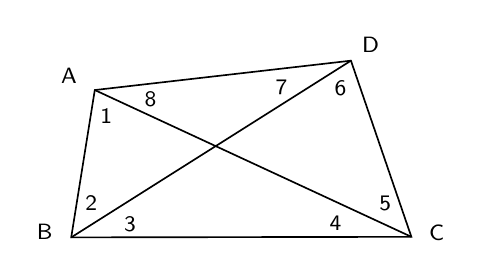
\begin{tikzpicture}[x=.72cm,y=.72cm,line width=.6pt,font=\footnotesize\sffamily]
 \coordinate (A) at (.416,2.599);
 \coordinate (B) at (0,0);
 \coordinate (C) at (6,.01);
 \coordinate (D) at (4.934,3.117);
 \draw (A)--(B)--(C)--(D)--cycle;
 \draw (A)--(C) (B)--(D);
 \node at (-.041,2.843) {A};
 \node at (-.467,.091) {B};
 \node at (6.447,.081) {C};
 \node at (5.279,3.401) {D};
 \node at (.619,2.132) {1};
 \node at (.355,.609) {2};
 \node at (1.035,.233) {3};
 \node at (4.66,.253) {4};
 \node at (5.54,.61) {5};
 \node at (4.75,2.63) {6};
 \node at (3.71,2.64) {7};
 \node at (1.40,2.44) {8};
\end{tikzpicture}
\end{center}
\[
\GaussRightBrace{\begin{array}{@{}l@{\;=\;}l@{}}
 \sin1\,.\sin3\,.\sin(6+7)&\sin(2+3)\,.\sin6\,.\sin8\\
 \sin3\,.\sin5\,.\sin(8+1)&\sin(4+5)\,.\sin8\,.\sin2\\
 \sin5\,.\sin7\,.\sin(2+3)&\sin(6+7)\,.\sin2\,.\sin4\\
 \sin7\,.\sin1\,.\sin(4+5)&\sin(8+1)\,.\sin4\,.\sin6.
\end{array}}\quad\text{\tikz[baseline=-.55ex,x=1mm,y=1mm,line width=.4pt]{\draw (0,1.2)--(-1.25,-.6)--(1.25,-.6)--cycle;\draw (0,-1.2)--(-1.25,.6)--(1.25,.6)--cycle;}}
\]

It is most advantageous to use the \(1^{\mathrm{st}},2^{\mathrm{nd}},3^{\mathrm{rd}}\) or \(4^{\mathrm{th}}\) form according as the triangle \(ABD,\allowbreak ABC,\allowbreak BCD,\allowbreak ACD\) is the largest.

It is not quite clear to me how you intended to use \raisebox{.8ex}{.}\,a measured diagonal direction\textsuperscript{[*)]}. The implication is that if six quantities \(A,B,C,D,E,F\) were measured, a condition equation
\[
 \partial A-\partial B+\partial C-\partial D+\partial E-\partial F=\text{Given quantity}
\]

\par\noindent\rule{4cm}{.4pt}\par
{\footnotesize\noindent\hspace*{\parindent}[*) \textsc{Gerling} believed that two further angle equations, each with a constant term of zero, had to be set up when one diagonal of a quadrilateral had been observed from only one end.]\par}
\noindent{\small IX.}\hfill{\small 32}\hspace*{.12\linewidth}\par

% Printed 250; principal PDF 257; Google PDF 261.
\par\clearpage
\noindent\makebox[0pt][l]{\fontsize{13}{16}\selectfont 250}\hfill{\small\textbf{CORRESPONDENCE.}}\hfill\null\par\medskip

\noindent would hold among their corrections, and now, since the sixth, \(F\), has \textls[120]{not} been measured, the condition equation
\[
 \partial A-\partial B+\partial C-\partial D+\partial E=0
\]
\noindent would have to hold. In fact, such a condition equation is wholly inadmissible, and adding the two you give would even yield something in direct contradiction with the rest.

All diagonal intersections can be taken into account only through \textls[120]{those} condition equations furnished by equations such as those marked above with \mbox{\tikz[baseline=-.55ex,x=1mm,y=1mm,line width=.4pt]{\draw (0,1.2)--(-1.25,-.6)--(1.25,-.6)--cycle;\draw (0,-1.2)--(-1.25,.6)--(1.25,.6)--cycle;}}. It makes no difference here whether or not the intersection was also observed reciprocally. In the first case alone the condition equation arising from the angle sum of one triangle is added (the equation for the other [triangle] is then already implicit in the others). This equation is absent in the other [case].

I repeat, incidentally, that everything is much simpler with the method I favored for my measurements. Furthermore, my own principal triangulation system contains no such diagonal that was not also measured reciprocally. I did not include in the system the few of this kind occurring on the boundaries, such as Hohehagen—Meisner, etc., and several new triangulation points, Syk and Hohenhorn. Instead, I have so far based all adjustment solely on the complete measurements, treating the other points as secondary points, so to speak, with respect to which the positions of my principal points are regarded as absolutely exact. . . . . . .

\bigskip
{\centering
\textsc{Gauss} to \textsc{Gerling}. \quad Göttingen, 19 January 1840.\par}
\medskip

. . . . . . Reading through your fine work on your \(\Delta\Delta\) has led me to think the matter through again a little, and a few remarks will probably be of some interest to you. Although I had predicted that you would obtain only slow convergence by treating the condition equations in zigzag fashion in two groups, I was nevertheless somewhat surprised that, according to one of your letters, you

% Printed 251; principal PDF 258; Google PDF 262.
\par\clearpage
\noindent\null\hfill{\small\textbf{ADJUSTMENT OF SIMPLE FIGURES.}}\hfill\makebox[0pt][r]{\fontsize{13}{16}\selectfont 251}\par\medskip

\noindent went through everything 15 times (13 times according to the book. I do not know how to explain this discrepancy). In my own arc-measurement system I had about 50 condition equations of the second kind and 12 of the third kind. Here, however, convergence was very rapid, so that by the third [calculation] the results were stable to \(\frac{1}{1000}''\). This would certainly have been impossible without a particular device that, it seems to me, you did \textls[120]{not} use. I do not know whether I pointed it out to you 15 years ago (in one of your letters you refer to communications made at the time), and I am also unsure whether I had already used it myself then. I believe my large adjustment calculations were made early in 1826, but I did not note a date anywhere. I will try to give you an idea of it, although a detailed development could make for a fairly substantial paper.

I assume, then, that the adjustment with respect to the condition equations depending on the angle sums has already been carried out once, and that one now wishes to proceed to the condition equations from the side ratios. For brevity I consider only a system of four points \(0\,.\,1\,.\,2\,.\,3\). If, of the four \(\Delta\Delta\), \(123\) is the largest, you use the formula \(\frac{01}{02}\,.\,\frac{02}{03}\,.\,\frac{03}{01}=1\) (here \(01\), etc., are sides, but from now on I denote by \(01\) the \textls[120]{angle} that this side makes with the zero line at \(0\)). That equation gives you \textls[120]{directly} a condition equation among \(9\) corrections, since \(\mathrm{d}01,\mathrm{d}02,\mathrm{d}03\) do not appear. Had you used the formula \(\frac{10}{12}\,.\,\frac{12}{13}\,.\,\frac{13}{10}=1\), you would have obtained a condition equation among \textls[120]{9 other} corrections, since \(\mathrm{d}10,\mathrm{d}12,\mathrm{d}13\) would have been absent. These two condition equations are therefore distinct, but one can be derived from the other by bringing in the condition equations of the second kind that belong to the quadrilateral. Here we encounter a case that often arises and to which a piece of advice that cannot be commended enough applies. When the components of an investigation are arranged symmetrically and the goal can be reached in more than one way, each apparently as good as the next, so that one is in the position of Buridan's ass, one should \textls[120]{choose none of these paths}, but seek another in which all the components receive equal treatment. Of course, no general rules can be given for
\par\smallskip
\noindent\hfill{\small 32\textsuperscript{*}}\hspace*{.12\linewidth}\par
